\documentclass[aps,twocolumn,secnumarabic,balancelastpage,amsmath,amssymb,nofootinbib]{revtex4}
\usepackage{amsmath}
\usepackage{amssymb}
\usepackage{amsfonts}
\usepackage{chapterbib}
\usepackage{color}
\usepackage{graphics}
\usepackage[pdftex]{graphicx}
\usepackage{grffile}
\usepackage{longtable}
\usepackage{epsf}
\usepackage{bm}
\usepackage{tikz}
\usepackage{asymptote}
\usepackage{thumbpdf}
\usepackage{bbm}
\usepackage{amscd}
\usepackage{units}
\usepackage{textcomp}
\usepackage[utf8x]{inputenc}
\usepackage{feyn}
\usepackage{feynmp}
\usepackage[colorlinks=true]{hyperref}
\newcommand{\drelectron}[1]{\node at #1 [circle, draw, inner sep=0pt, minimum size=1pt] {\_}}

\newcommand{\ud}{\mathrm{d}}
\newcommand{\ue}{\mathrm{e}}
\newcommand{\ui}{\mathrm{i}}
\newcommand{\res}{\mathrm{Res}}
\newcommand{\Tr}{\mathrm{Tr}}
\newcommand{\dsum}{\displaystyle\sum}
\newcommand{\dprod}{\displaystyle\prod}
\newcommand{\dlim}{\displaystyle\lim}
\newcommand{\dint}{\displaystyle\int}
\newcommand{\fsno}[1]{{\!\not\!{#1}}}
\newcommand{\eqar}[1]
{
  \begin{align*}
    #1
  \end{align*}
}
\newcommand{\eqarn}[1]
{
  \begin{align}
    #1
  \end{align}
}
\newcommand{\texp}[2]{\ensuremath{{#1}\times10^{#2}}}
\newcommand{\dexp}[2]{\ensuremath{{#1}\cdot10^{#2}}}
\newcommand{\eval}[2]{{\left.{#1}\right|_{#2}}}
\newcommand{\paren}[1]{{\left({#1}\right)}}
\newcommand{\lparen}[1]{{\left({#1}\right.}}
\newcommand{\rparen}[1]{{\left.{#1}\right)}}
\newcommand{\abs}[1]{{\left|{#1}\right|}}
\newcommand{\sqr}[1]{{\left[{#1}\right]}}
\newcommand{\crly}[1]{{\left\{{#1}\right\}}}
\newcommand{\angl}[1]{{\left\langle{#1}\right\rangle}}
\newcommand{\tpdiff}[4][{}]{{\paren{\frac{\partial^{#1} {#2}}{\partial {#3}{}^{#1}}}_{#4}}}
\newcommand{\tpsdiff}[4][{}]{{\paren{\frac{\partial^{#1}}{\partial {#3}{}^{#1}}{#2}}_{#4}}}
\newcommand{\pdiff}[3][{}]{{\frac{\partial^{#1} {#2}}{\partial {#3}{}^{#1}}}}
\newcommand{\diff}[3][{}]{{\frac{\ud^{#1} {#2}}{\ud {#3}{}^{#1}}}}
\newcommand{\psdiff}[3][{}]{{\frac{\partial^{#1}}{\partial {#3}{}^{#1}} {#2}}}
\newcommand{\sdiff}[3][{}]{{\frac{\ud^{#1}}{\ud {#3}{}^{#1}} {#2}}}
\newcommand{\tpddiff}[4][{}]{{\left(\dfrac{\partial^{#1} {#2}}{\partial {#3}{}^{#1}}\right)_{#4}}}
\newcommand{\tpsddiff}[4][{}]{{\paren{\dfrac{\partial^{#1}}{\partial {#3}{}^{#1}}{#2}}_{#4}}}
\newcommand{\pddiff}[3][{}]{{\dfrac{\partial^{#1} {#2}}{\partial {#3}{}^{#1}}}}
\newcommand{\ddiff}[3][{}]{{\dfrac{\ud^{#1} {#2}}{\ud {#3}{}^{#1}}}}
\newcommand{\psddiff}[3][{}]{{\frac{\partial^{#1}}{\partial{}^{#1} {#3}} {#2}}}
\newcommand{\sddiff}[3][{}]{{\frac{\ud^{#1}}{\ud {#3}{}^{#1}} {#2}}}

\begin{document}
\tikzstyle{every picture}+=[remember picture]
\title{Simulation of Raman sideband cooling with large Lamb-Dicke factor and high initial temperature}
\author{Yichao Yu}
\email{yuyichao@mit.edu}
\homepage{http://yyc-arch.org/}
\date{\today}
\affiliation{MIT Department of Physics}

\begin{abstract}
  It is usually believed that Raman sideband cooling requires a particle to be confined to much smaller than the optical wavelength, i.e. small Lamb-Dicke factor and low initial vibrational state, in order to suppress the heating from light scattering. In this paper, I will show with numerical simulation of the optical Bloch equation that by driving Raman transitions between vibrational states with $\delta n\gg1$, it is possible to preform Raman sideband cooling with a big Lamb-Dicke factor ($\eta=0.8$) and a high initial temperature $k_BT/\hbar\omega=30$.
\end{abstract}

\maketitle
%%%%%%%%%%%%%%%%%%%%%%%%%%%%%%%%%%%%%%%%%%%%%%%%%%%%%%%%%%%%%%%%%%
\section*{Introduction}
Sideband cooling is a powerful technique for cooling confined particles, especially for ions in ion traps, to their ground states in both external and internal degrees of freedom. One of its variation, is also used in some experiment for cooling neutral atoms confined in an optical lattice\cite{sideband-cs-lattice} or a tightly focused tweezer optical dipole trap\cite{sideband-single-jila,sideband-single-cua}. Due to the heating from photon scattering, most of these experiments requires the particle to be confined to much smaller than an optical wavelength. Although this is possible to do for heavy atoms, e.g. Rubidium and Cesium, or ions, it is hard to get the same confinement for lighter neutral atoms like sodium.

\section{Simulation using Optical Bloch Equation}
\begin{figure}
  \begin{center}
    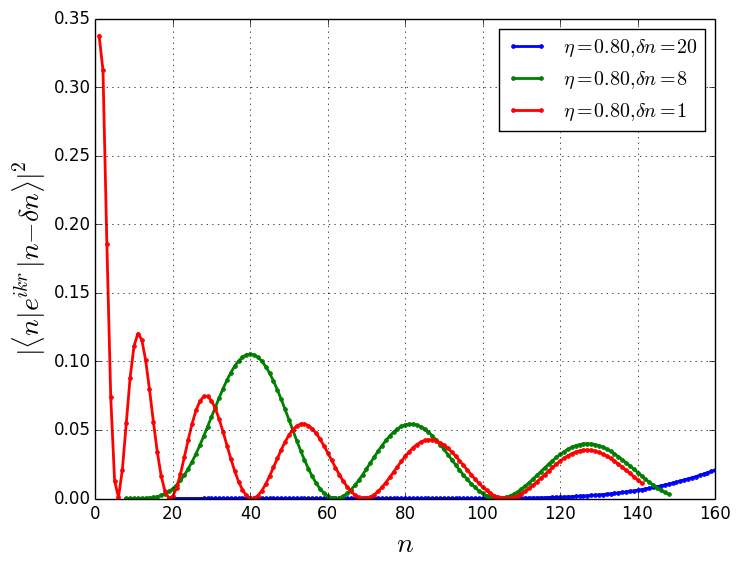
\includegraphics[width=7cm]{../raman_0.8_1.png}
  \end{center}
  \caption{Coupling strength to lower vibrational state for different initial states.}
  \label{fig-raman-curve}
\end{figure}
\begin{figure}
  \begin{center}
    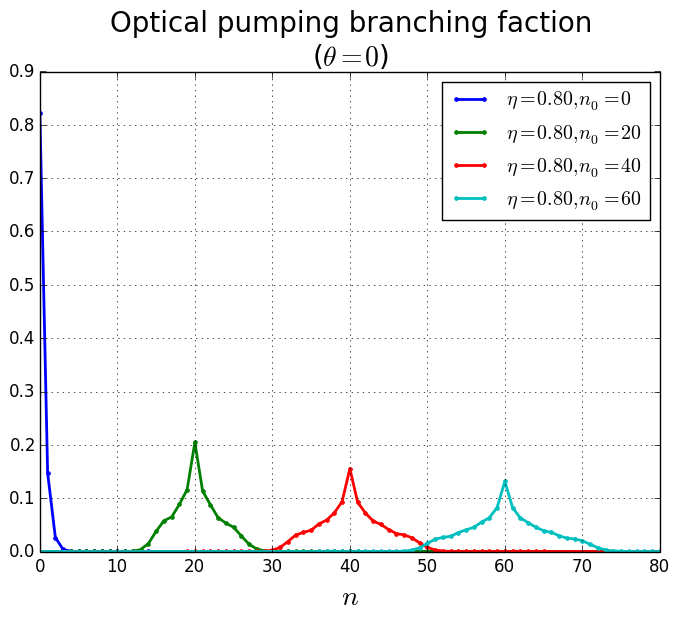
\includegraphics[width=7cm]{../pump_0.8_0_curve.png}
  \end{center}
  \caption{Possibilities of going in to other vibrational states (i.e. heating) during optical pumping. The pumping beam is sent in from the orthogonal direction.}
  \label{fig-pump-curve}
\end{figure}

\section{Results of the simulation}
\begin{figure}
  \begin{center}
    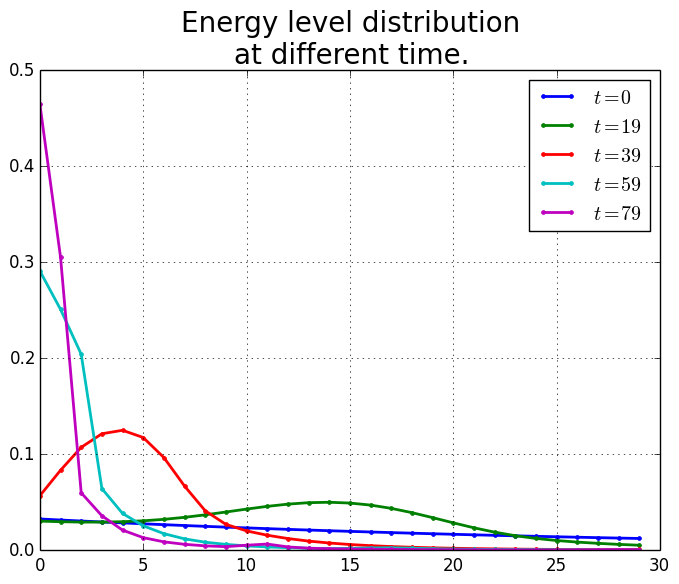
\includegraphics[width=7cm]{../cool_process.png}
  \end{center}
  \caption{Distribution in vibrational levels (including both hyperfine ground states) at different time. States with $n>30$ are not shown in the figure.}
  \label{fig-cool-process}
\end{figure}
\begin{figure}
  \begin{center}
    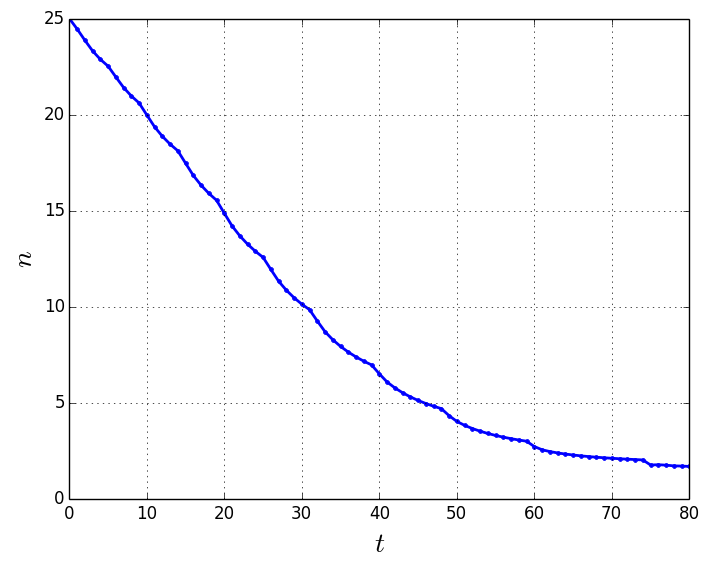
\includegraphics[width=7cm]{../n_decrease.png}
  \end{center}
  \caption{Decrease of $n$ during the cooling process.}
  \label{fig-n-decrease}
\end{figure}

\section{Conclusion.}

\bibliography{paper}
\end{document}
